\section{Materials and methods}
For this study, we generated 4 different datasets with molecular docking scores (datasets AA2AR\_1/2 and CB2\_1/2), and used 2 datasets available in open-source \cite{ultralarge_docking_first} (datasets AmpC and D4). Score distribution is shown on Fig. \ref{fig:fig_1}.

\subsection{Molecular docking}
To obtain scores for AA2AR\_1/2 and CB2\_1/2, we performed molecular docking in ICM-Pro molecular modeling software (ver. 3.9.1). Namely, we used high-resolution X-ray crystal structures of human cannabinoid receptor 2 (CB2, PDB ID 5ZTY) and adenosine receptor A2 (AA2AR, PDB ID 4EIY). Models were prepared as described in the Molsoft ICM user guide \cite{molsoft_guide}. Namely, we loaded them into ICM-Pro package, removed ligands and converted the receptor models into an ICM format using default settings, which includes building missing side chains, adding hydrogens, energy-based Gln/Asn/His conformation optimization, and removal of all water molecules. Docking box was selected around co-crystallized ligands.

As a screening library, we used randomly selected $1\ 000\ 000$ drug-like ($200 < \texttt{MW} < 500$, $\texttt{logP} < 5$) compounds from ZINC20 database \cite{Irwin2020ZINC20Discovery} . We converted compounds from SMILES to three-dimensional SDF  format, added hydrogen atoms and assigned formal charges at pH=7.0 (according to ICM pKa model implemented in ICM-Pro).

Docking was performed using ICM-Pro package without receptor flexibility, and with ligand sampling thoroughness (effort) 1.0.

\subsection{Preparation of supervised learning dataset}
Molecular docking scores were downloaded from Figshare (for AmpC and D4 datasets) or obtained from resulting SDF files with the best ligand pose (for AA2AR and CB2 datasets). For AmpC and D4, we selected random subsets of 1 million molecules using `shuf scores.txt | head -n 1000000` command in Linux. Then, we generated Morgan fingerprints (size 2048, radius 2) using $\texttt{chemfp}$ \cite{Dalke2019} for all molecules from their SMILES strings, and concatenated with their respective docking scores to obtain final supervised learning datasets with fingerprints as features and scores as values for prediction. Docking score distributions are shown on Figure \ref{fig:fig_1}.


\subsection{Single-shot prediction of virtual screening hits}
We tested classic machine learning algorithms for their ability to predict virtual screening hits (VSH). Namely, we labeled top-1\% of the ligands in datasets AmpC, D4, AA2AR\_1 and CB2\_1 as hits, and the rest as non-hits, and tested machine learning algorithms in their ability to recover VSHs from the ligand pool after training on a small subset of molecules with their scores. We deliberately choose a large percentage, top-1\%, compared to the earlier works \cite{Graff2021AcceleratingLearning, logistic_regression, Yang2021_shoichet_active_learning} due to the small size of the library in order to decrease the subsequent deviation of the performance metric.

As for algorithm selection, we choose both "lightweight" and "heavy" models in both regression (predicting the docking score from molecule's Morgan fingerprint directly) and classification (predicting label of each ligand) regimes. Namely, we tested following models (as named in scikit-learn library): LinearRegressor, Ridge/RidgeCV, LinearSVR, KNeighboursRegressor (with 1 and 5 neighbours), KNeighboursRegressor (with Jaccard metric), DecisionTreeRegressor, RandomForestRegressor, KNeighboursClassifier (with 5 neighbours), DecisionTreeClassifier, and SGDClassifier. All models were imported from scikit-learn Python library \cite{scikit-learn} (ver. 0.23.2). 

For cross-validation, we performed 5-fold stratified cross-validation. Namely, for each train size $n$ we selected $1.2n$ ligands for each fold, labeled top-1\% as hits and used stratified 5-fold split. This way, models were trained on $n$ ligands and tested on $n/5$ ligands, with $1:99$ imbalance in both train and test sets.

For performance measure, we used model recall: number of true VHSs in top-1\% of ligands in validation set, sorted by predicted docking score.

For AA2AR and CB2 datasets we also constructed lower- and upper-bound baselines. A random number generator, either uniform or gaussian, matching the overall score distribution, was chosen as lower-bound baseline. A docking score from the second docking with the same receptor was chosen as an upper-bound baseline, assuming that no machine learning model can provide us with a better docking score than docking itself. The uniqueness of scores is ensured by the stochastic nature of obtained docking scores, based on the ligand sampling algorithm \cite{abagyan_biased_1994}.

\subsection{Single-shot results extrapolation}

After obtaining results for single-shot model performance, we went to explore the active learning regime. In this regime, a \textit{base model} is trained at each step, and its predictions are than docked at the next step, instead of randomly chosen ligands. First, we estimated the effect of batch size on the overall virtual screening performance in the active learning regime. In order to do that, we compared few scenarios: 
\begin{enumerate*}[label=(\roman*)]
    \item memory-less active learning model with LinearRegression as a base model;
    \item extrapolation of a single-shot prediction, under assumption that recall remains constant;
    \item lower-bond baseline of random docking score assignment;
    \item upper-bond baseline, picking docking score from a second docking attempt (for AA2AR and CB2 datasets).
\end{enumerate*}

In each scenario, a base learning model was initially trained on random $\texttt{batch\_size}$ ligands with their scores. This model than was used to pick next $\texttt{batch\_size}$ ligands from the rest of the set (as top-1\% of the ligands, ranked by their predicted docking score). Then, the next base model was trained on the scores of ligands from the previous iteration, and so on.

In order to extrapolate single-shot model performance, we assumed that the model performance doesn't change with the deterioration of the ligand pool, and recall remains the same. Given batch size $n$, total number of ligands $N$, recall $r$ and hits fraction $\beta=0.01$, at iteration 0 model retrieves $h_0 = n\beta$ VHSs. At iteration $j$, model retrieves fraction $r$ of the remaining VHS: $h_j = ( N\beta - \sum_{i=0}^{j-1}h_i ) \cdot r$. Subsequently, the total number of hits retrieved by step $j$ is $H_j = \sum_{i=0}^{j} h_i$.

To evaluate performance of the active learning regime, we calculated number of retrieved VSHs. For each batch size and dataset, we performed 3 attempts, using the same fold labels between different batch sizes.

\subsection{Active learning regime parameters}

After testing the batch size effect and reliability of constant recall extrapolation, we explored different scenarios of the active learning regime. Namely, we tried
\begin{enumerate*}[label=(\roman*)]
    \item different batch sizes;
    \item exploiting models from earlier ($i < j$) iterations at iteration $j$, with different methods of ensembling of multiple models;
    \item adding previously discovered ligands to the train set at step $j$, hence making train set size at step $j$ $|X_j| = nj$ instead of $|X_j|=n$.    
\end{enumerate*}

Similarly to the previous section, we used here LinearRegression as base model, given its small training and inference time, as well as its consistently good performance on all datasets. Also, for AA2AR and CB2 datasets, we used second docking as an upper-bond baseline. Finally, we used random score assignment as lower-bond baseline in all 4 datasets. 

Also, similarly to the previous section, we used model recall, i.e. the amount of VSHs retrieved by the active learning model, as a performance metric.

For model ensembling, we used 3 different regimes. LastModel used no ensembling altogether, accounting only for the latest model predictions. MeanRank for each ligand assigned rank $p_i$ by model $i$, and used $\langle p_i \rangle$ as a ligand score. Finally, TopFromEveryModel used smaller portion of each model's top ($k$ times smaller for $k$ different models), and compiled individual tops into an ensemble prediction.

%% --------------------------------

\begin{figure}[h]
\centering
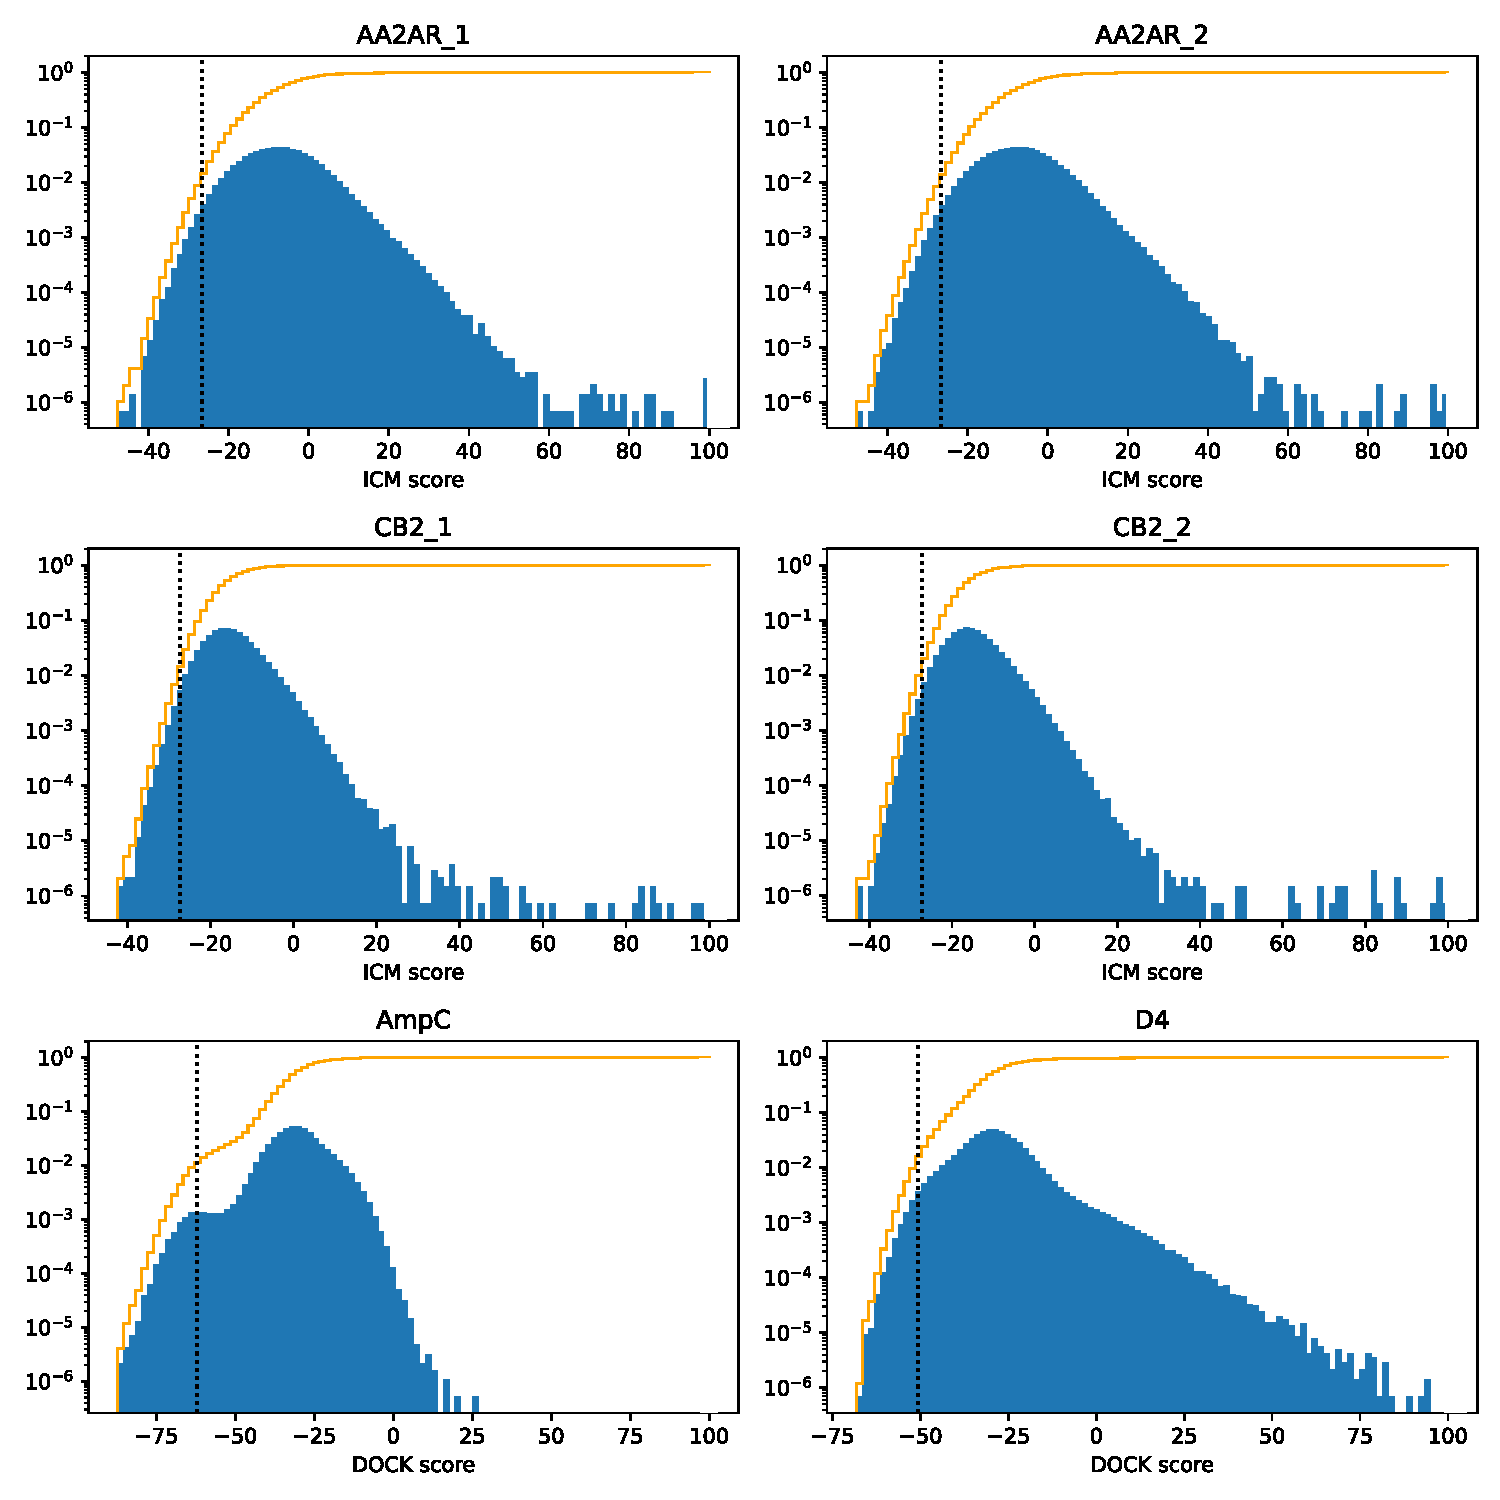
\includegraphics[width=0.8\textwidth]{figures/scores_distribution_v3.pdf}
\caption{Distributions of scores for datasets used in the study. Histogram (blue) shows log-scale score distribution, while plot (orange) shows cumulative distribution of scores. Vertical line (black) shows cutoff for top-1\% of scores. TODO: \textit{change Dock to DOCK}}
\label{fig:fig_1}
\end{figure}


\begin{figure}[h]
\centering
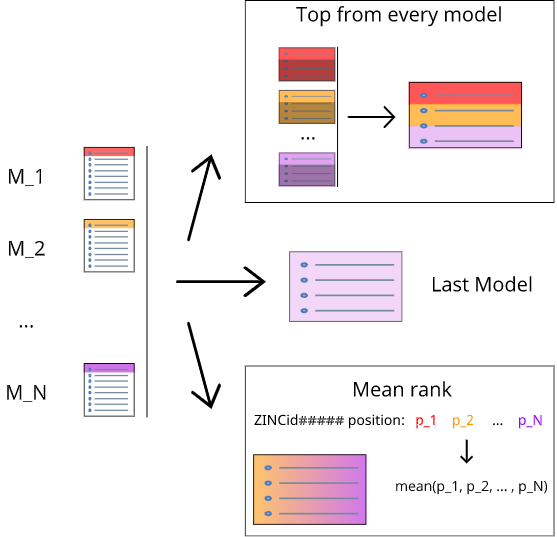
\includegraphics[width=0.8\textwidth]{figures/Figure_N_iteration_methods.png}
\caption{Overview of the active learning ranking schemes. \textit{TODO: make them CamelCaseTitles, very likely -- re-draw (arrows ugly, alignment sucks)}}
\label{fig:fig_2_scheme}
\end{figure}



% \subsection{Prediction of docking scores} \label{subsec:prediction}

% Current work consists of two parts: evaluation of the quality of an individual machine learning model and examination of iterative algorithm efficiency depending on its hyperparameters.
% Train and tests datasets are required for both parts.
% For machine learning pipeline, results of molecular docking with adenosine and cannabinoid receptors were used, as well as docking scores from \cite{ultralarge_docking_first} for AmpC $\beta$-lactamase and $\text{D}_4$ dopamine receptor.
% To obtain feature vectors for each molecule in the screening library, binarised Morgan fingerprints of size 2048 were generated using chemfp.

% \subsubsection{Utilised models}

% The following classifiers and regressors from the scikit-learn machine learning library were tested:
% \begin{itemize}
%     \item Linear regression;
%     \item Ridge (and RidgeCV);
%     \item Lasso (and LassoCV);
%     \item Linear SVR;
%     \item KNeighbours regressor (with one and five neighbours);
%     \item KNeighbours regressor with Jaccard metric;
%     \item DecisionTree regressor;
%     \item RandomForest regressor;
%     \item KNeighbours classifier (with five neighbour);
%     \item DecisionTree classifier;
%     \item RandomForest classifier;
%     \item SGD classifier.
% \end{itemize}

% All models were imported from scikit-learn Python library and trained over 5 cross-validation repeats with different set sizes (8000, 40000, 80000, 160000 and 320000 compounds).
% Besides, classifiers were trained on different types of binarised scores depending on the percentage of the docking hits (0.5\%, 1\%, 2\% or 5\%).

% To understand how great or poor the performance of the ML models is, two types of reference models were used.
% First model is second docking performed with effort=1, and it is supposed that it gives gives the upper bond: none ML model can outperform docking. 
% Due to stochastic nature of sampling in ICM-Pro, it gives slightly different results every time, if the random seed is not fixed.
% The lower bound is taken from so-called "dummy" regressors and classifiers: model returning random values according to normal or uniform distribution was utilized as a dummy regressor, and a classifier which simply returns the most frequent class was chosen to be dummy classifier.

%quality metric?

% \subsubsection{Iteration scheme}

% In iterative algorithms, only regression methods were used.
% The pipeline of the algorithm consists of the following steps:
% \begin{enumerate}
%     \item In the initial step, a predefined number of molecules are "docked" (practically, taken from the list of already docked compounds) to provide a test set;
%     \item The ML model is trained and integrated then into a complex model;
%     \item The complex model predicts the docking outcome;
%     \item The batch of molecules is docked: if the number of docking hits is larger than a predefined size, then the demanded number of hits are sampled;
%     In the opposite situation, randomly sampled molecules from non-hits are added to all docking hits in order to gain the required amount;
%     \item Depending on the algorithm protocol (Fig. \ref{TrainSetSelection}), the batch from the precious step is either added to the train dataset, or is utilized as a train dataset itself;
%     \item Steps 2-5 are repeated until the predetermined number of iteration is reached.
% \end{enumerate}

% There are two ways to update train dataset from iteration to iteration.
% On the one hand, it is profitable to make use of all the docked molecules, because more information is gathered.
% Most likely that single models in one round of iteration algorithm will be similar to each other and prioritize the molecules which properties close to each other.
% On the other hand, the selection of only the latest batch of docked molecules for training may cause more diversity in single models' parameters.
% Thus, models from different step will search for docking hits in various parts of chemical space.
% Both approaches were tested within the iterative algorithms.

% Three types of complex models were employed in the algorithm:
% \begin{itemize}
%     \item \textbf{Last Model}: ML model from the latest iteration is treated as a complex model and used to predict docking outcomes.
%     After the prediction, top-k\% of predicted scores become hits;
%     \item \textbf{Top from every model}: on the $\text{n}^{th}$ iteration, each model makes a prediction and top-(k/n)\% of predicted scores from each model constitute complex model's hits (duplicates are deleted);
%     \item \textbf{Mean Rank}: for each compound, the positions in the ratings of all models are averaged; the k\% of the compounds with the smallest average positions are handled as hits.
% \end{itemize}

%quality metric?


% how we did machine learning
% ? Fig 2: machine learning pipelines
% 	- A: cross-validation scheme for "best model" figure
% 	- B: cross-validation scheme for iterations
% 	- what "iterations" mean & their different regimes (from diploma)

